\chapter{Testování výsledků}
\label{chap:evaluace}

Výsledný program se skládá z~několika komponent. Funkčnost každé komponenty lze testovat. Některé části je možné otestovat automaticky, například rozpoznávání jazyka. Na některé části je potřeba testování s uživateli.

Klíčovou částí celého projektu je algoritmus, který k~textu přiřadí ilustrační obrázek. Úspěšnost tohoto algoritmu byla otestována na uživatelích. Rozhraní může fungovat pro~více jazyků. Testování však proběhlo pro~vstupní texty v~češtině. Výhodou je snadnější získání anotátorů v~českém jazyce. Hlavním důvodem je ovšem pravděpodobná vyšší nepřesnost algoritmu v~češtině. Dataset Profimedie má data v~anglickém jazyce a pro~české použití musel být přeložen. Pokud se tedy ukáže, že algoritmus funguje dobře pro~češtinu, měl by pro~angličtinu fungovat ještě lépe. pro~testování bylo využito testovací rozhraní popsané v~Kapitole~\ref{chap:rozhrani}.


\section{Vyloučení narušitele (o\_test1)}

\begin{figure}[h]
  \centering
  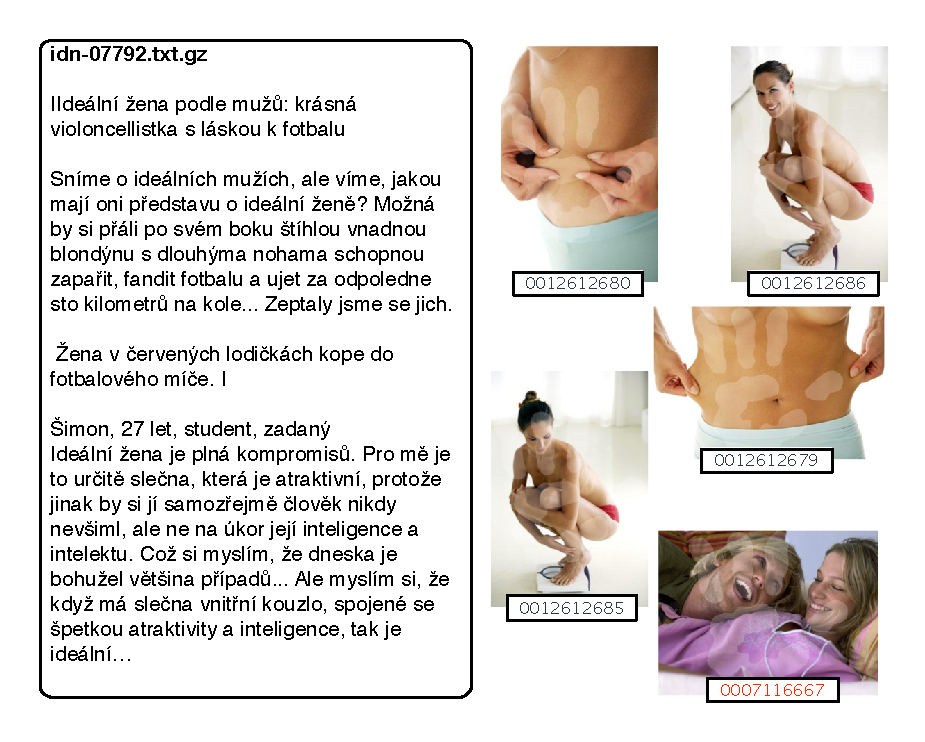
\includegraphics[width=150mm]{evaluace_1.eps}
  \caption{Ukázka testu vyloučení narušitele pro~článek idn-07792.}
  \label{fig:evaluace_1}
\end{figure}


První metodou testování bylo \uv{vyloučení nepřítele} (anglicky \uv{intruder detection}). Tato metoda se používá k~evaluaci automaticky detekovaných shluků slov a je popsána například v~\cite{chang}. v~naší variantě se evaluují obrázky přiřazené k~textu. Nejprve se k~danému textu najdou pomocí testovaného algoritmu 4 nejvíce odpovídající obrázky. k~nim se přidá jeden náhodně vybraný obrázek z~datasetu a poté se náhodně zamíchá pořadím těchto obrázků. Anotátor vidí v~anotačním rozhraní text a 5 obrázů. Jeho úkolem je označit obrázek, který danému textu podle jeho názoru odpovídá nejméně. Pokud algoritmus přiřazující obrázky textu funguje správně, měl by být uživatel schopen označit obrázek, který byl do~sady vybrán náhodně a rozlišit ho od obrázků, který vybral algoritmus přiřazující obrázky.

Texty pro~testování algoritmu pochází z~korpusu online článků stažených z~českých webových serverů. Jedná se o články, které obsahují ilustrační obrázky z~datasetu Profimedie. Takto omezená množina novinových textů je pro~náš účel velmi výhodná. pro~různé druhy článků dataset Profimedie neobsahuje žádné vhodné ilustrační obrázky. Jedná se například o politické zpravodajství, pro~které v~datasetu aktuální fotky událostí nebo například archivní fotky osobností. Oproti tomu u článků, které již nějaký ilustrační obrázek z~Profimedie obsahují, jsou možnosti vhodného obrázku daleko vyšší. Jedná se většinou o hobby a společenské články.

Pro naše testování jsme využili články ze serveru iDnes\footnote{\url{http://www.idnes.cz}}, který obsahoval nejvíce článků s ilustračními obrázky z~Profimedia. Konkrétně jich máme k~dispozici $4223$.

Z těchto $4 223$ článků jsme náhodně vybrali pro~testování 60 článků. Ke každému z~článků byly získány algoritmem 4 doporučené ilustrační obrázky a byl přidán jeden obrázek náhodný. Každá tato testovací sada byla otestována dvěma anotátory. Bylo k~dispozici 5 anotátorů. Dohromady to znamenalo pro~každého anotátora 24 a dohromady 120 anotací. Anotace byly rozděleny tak, aby každá dvojice anotátorů měla právě 6 stejných testovacích sad.

Během anotace se zjistilo, že u dvou testovacích sad se jeden z~obrázků nenačítá. Tyto sady byly z~testování vyřazeny a anotovaných testovacích sad je tedy pouze 58. Výsledky testování jsou shrnuty v~tabulce~\ref{tab:testresults} ve~sloupci \uv{o\_test1}. Pobrobné výsledky testování včetně Cohenovy kappy pro~všechny dvojice anotátorů jsou v~příloze~\ref{app:testing}.

Výsledky ukazují, že pro~78~\% testovacích sad měli anotátoři pozitivní shodu. Pozitivní shoda znamená, že se oba anotátoři shodli na stejném obrázku, který je pro~vstupní text nejméně vhodný. Tento obrázek byl zároveň vybrán do~testovací sady náhodně. Čím je toto procento vyšší, tím lépe náš algoritmus pracuje, protože uživatelé jsou schopní detekovat náhodný obrázek. pro~5~\% testovacích sad máme negativní shodu. Oba anotátoři vybrali obrázek, který nebyl přiřazen náhodně. Znamená to tedy, že tento obrázek nebyli schopní detekovat a algoritmus tedy pro~vstupní text nepracuje dobře (pokud vyloučíme možnost, že náhodně přiřazený obrázek je k~textu relevantní). U poslední skupiny testovacích dat -- 17~\% -- byl pouze jeden z~anotátorů schopen vybrat náhodně vybraný obrázek. 

\begin{table}
\label{tab:testresults}
\centering
\begin{tabular}{ | l || r | r | r |}
  \hline
     & \multicolumn{1}{c |}{\textbf{o\_test1}} & \multicolumn{1}{c |}{\textbf{o\_test2}} & \multicolumn{1}{c |}{\textbf{celkem}} \\
  \hline
  \hline
    \textbf{anotátorů} & 5 & 5 & 7 \\
  \hline
    \textbf{textů} & 58 & 120 & 178 \\
  \hline
    \textbf{anotací} & 116 & 240 & 356 \\
  \hline
    \textbf{pozitivní shoda} & $45/58=78\%$ & $76/120=\mathbf{63}\%$ & $121/178=67\%$ \\
  \hline
    \textbf{negativní shoda} & $3/58=5\%$ & $15/120=13\%$ & $18/178=10\%$ \\
  \hline
    \textbf{neshoda} & $10/58=17\%$ & $29/120=24\% $ & $39/178=22\%$ \\
\hline
\end{tabular}

  \caption{Přehled výsledků uživatelského testování.}
\end{table}

Získaná data ukazují, že algoritmus pracuje poměrně správně. Pokud by algoritmus přiřazoval automaticky obrázky k~textům i v~praxi, čtenáři by byli schopní výstupy tohoto algoritmu odlišit od algoritmu, který přiřazuje obrázky k~textům náhodně.

Během testování se objevil jeden zásadní problém s testovací metodou. v~datasetu Profimedie jsou i obrázky, které jsou si velmi vizuálně podobné, například fotky stejné osoby z~různých úhlů. Tyto fotky mají často i stejné textové popisky. Mějme tedy 4 obrázky, které jsou si vizuálně velmi podobné a mají stejné textové popisky. Pokud algoritmus označí jako nejvhodnější obrázek k~textu jeden z~těchto obrázků, budou i na dalších třech doporučených pozicích vizuálně podobné obrázky (pokud tedy nemáme jinou množinu obrázků, která má stejné textové popisky, ale je vizuálně odlišná). Pokud se takový text objeví v~naší testovací metodě, uvidí anotátor 4 velmi podobné obrázky a k~nim jeden náhodně vybraný. Nejméně vhodný obrázek pak snadno označí, aniž by vůbec četl anotační text. Ukázalo se, že v~našem testování k~takovému problému opravdu došlo -- anotátorovi se zobrazily obrázky, z~nichž ani jeden nebyl vhodným obrázkem k~danému textu, přesto anotátor snadno označil nejméně vhodný obrázek. Tento problém může zkreslovat výsledky testování touto metodou.

Dobře je tento problém vidět na ukázce anotace v~Obrázku~\ref{fig:evaluace_1}. Text článku je anketa mezi muži o ideální ženě. Obrázek ze sady fotek s tématem hubnutí by asi nebyl úplně ideální ilustrační obrázek k~danému článku. Možná že náhodně přidaný obrázek s~id \uv{0007116667} by článek ilustroval lépe. Oba anotátoři ho však označili za~nejméně vhodný, protože ostatní obrázky jsou ze stejné série.

Zajímavé je analyzovat, proč obrázky s tématikou hubnutí přiřadil algoritmus jako vhodné k~článku o ideální ženě. Algoritmus v~článku označil jako klíčová postupně slova \uv{ideální}, \uv{žena}, \uv{let}, \uv{svobodný} a \uv{ráda}. První nalezený obrázek má id \uv{0012612680}. Slovo \uv{ideální} se v~českém překladu nachází dvakrát (z překladu frází \uv{ideal figure} a \uv{ideal body measurements}). Dvakrát se v~klíčových slovech obrázku nachází \uv{žena}. Stejně tak slovo \uv{let} z~anglického \uv{years}, které není pro~daný obrázek příliš relevantní. Slovo \uv{svobodný} se do~českých metadat obrázku dostalo nesprávným překladem. Anglická metadata obrázku obsahují frázi \uv{skin folds upper body freely}. Slovo \uv{freely} by v~takovém kontextu mělo být přeloženo spíše jako \uv{volný} než jako \uv{svobodný}. Obrázek s id \uv{0012612680} ukazuje velkou část problémů, které algoritmus vyhledávání ilustračních obrázků k~textu má, zejména s přeloženými texty.


\section{Detekce správného obrázku (o\_test2)}

Abychom předešli problémům s metodou popsaným v~předchozí sekci, provedli jsme nové testování. Úkolem uživatelů bylo nyní vybrat obrázek, který se ke vstupnímu textu hodí nejvíce. Množinu obrázků nyní tvořil jeden výstup z~algoritmu a 4 náhodně vybrané obrázky. Zvětšili jsme i testovací sadu. Bylo testováno 120 textů náhodně vybraných z~iDnes datasetu. Každý z~textů byl anotován dvěma anotátory. Na každém z~pěti anotátorů tedy bylo 48 anotací. Výsledky testování jsou shrnuty v~Tabulce~\ref{tab:testresults} ve~sloupci \uv{o\_test2}. Pobrobné výsledky testování, včetně Cohenovy kappy pro~všechny dvojice anotátorů je v~příloze~\ref{app:testing}.

Výsledky jsou oproti předchozí metodě o něco horší. pro~63~\% testovacích sad měli oba anotátoři pozitivní shodu, pro~13~\% měli anotátoři negativní shodu a pro~24~\% se anotátoři neshodli.

Zajímavý je rozbor anotací, u kterých správný obrázek neuhodl ani jeden z~obrázků. Některé nesprávně označené výsledky jsou způsobeny špatnou volbou náhodných obrázků. v~anotaci textu \uv{idn-01911} ukázané na Obrázku~\ref{fig:evaluace_2_1} o~novém softwarovém centru společnosti Microsoft se náhodně objevili 3 obrázky na kterých je počítač.

\begin{figure}[h]
  \centering
  \includegraphics[width=130mm]{evaluace_2_1.eps}
  \caption{Obrázky v~evaluaci textu idn-01911. Algoritmem doporučený je 2. obrázek v~pořadí.}
  \label{fig:evaluace_2_1}
\end{figure}


Podobný problém má anotace na Obrázku~\ref{fig:evaluace_2_1}, kde se u článku o úbytku plochu polí a zvětšování plochy lesů objevily náhodně obrázky pole a lesa. Tyto problémy při testování algoritmu by šly odstranit lepším výběrem náhodných obrázků. Například by obrázky mohly být náhodně vybrány z~množiny, která neobsahuje žádné z~doporučených klíčových slov textu.

\begin{figure}[h]
  \centering
  \includegraphics[width=130mm]{evaluace_2_2.eps}
  \caption{Obrázky v~evaluaci textu idn-02505. Algoritmem doporučený je 4. obrázek v~pořadí.}
  \label{fig:evaluace_2_2}
\end{figure}

Někdy jsou špatné výsledky způsobeny chybným nastavením důležitosti jednotlivých klíčových slov. Obrázek~\ref{fig:evaluace_2_3} ukazuje obrázky u anotace článku o povýšení a kariéře žen. Algoritmus pro~detekci klíčových slov správně určil jako první klíčové slovo \uv{ženy}. Na dalších pozicích jsou \uv{manažerských}, \uv{muže}, \uv{řídících} a \uv{zaměstnání}. Doporučený obrázek kromě klíčového slova \uv{ženy} obsahuje všechna ostatní detekovaná klíčová slova. Anotátoři však měli ve~výsledcích obrázek se ženou, kterému dávali přednost.

\begin{figure}[h]
  \centering
  \includegraphics[width=130mm]{evaluace_2_3.eps}
  \caption{Obrázky v~evaluaci textu idn-04282. Algoritmem doporučený je 3. obrázek v~pořadí.}
  \label{fig:evaluace_2_3}
\end{figure}


Problémem se ukázaly být také příliš krátké popisky obrázků. Obrázek~\ref{fig:evaluace_2_4} ukazuje anotační obrázky pro~text vracení záloh za~elektřinu. Třetí obrázek má v~klíčových slovech jediné slovo \uv{backup}, které je přeloženo jako \uv{záloha}. Vyhledávací algoritmus preferuje ve~výsledcích obrázky s kratšími popisky klíčových slov, takže se tento obrázek s jednoslovným popisem stal doporučeným k~danému textu. Zdá se z~více případů, že tyto obrázky s velmi krátkými popisky by mohly být pro~lepší výsledky z~vyhledávání odstraněny.

\begin{figure}[h]
  \centering
  \includegraphics[width=130mm]{evaluace_2_4.eps}
  \caption{Obrázky v~evaluaci textu idn-04368. Algoritmem doporučený je 3. obrázek v~pořadí.}
  \label{fig:evaluace_2_4}
\end{figure}

\section{Shrnutí}

Uživatelské testování ukazuje, že je algoritmus schopen v~poměrně velkém procentu případů přiřadit automaticky \uv{dostatečňě vhodný} ilustrační obrázek. To, že je ilustrační obrázek dostatečně vhodný ovšem neznamená, že je nejvhodnější. Výběr nejvhodnějšího ilustračního obrázku je ovšem velmi individuální a nedá se obecně měřit. Při testování se ukázalo, že některé náhodně vybrané obrázky, byly anotátory označeny jako lepší ilustrační obrázky pro~daný text, než obrázky automaticky přiřazené algoritmem. To ovšem neznamená, že by tyto obrázky byly vždy pro~daný test nevhodné. Ukazuje se, že některé druhy textů mohou obsahovat poměrně širokou škálu přijatelných ilustračních obrázků.

Testování ukázalo také na slabiny algoritmu. Možná největší slabinou je fáze překladu, díky níž popisky k~některým obrázkům nesprávné. Tímto problémem netrpí algoritmus pro~anglické vyhledávání, který pracuje s nepřeloženými popisky. Další množina problémů je způsobena nesprávnými popisky u obrázků. Některé obrázky jsou popsány desítkami klíčových slov, jiné zase pouze jedním.

Jedním z~problémů našeho testování je omezená doména testovaných textů. Můžeme říci, že algoritmus funguje dobře na nějaké doméně textů, ale pro~obecné zpravodajské články může algoritmus fungovat velmi špatně. Toto ovšem není problém testovaného algoritmu, ale dat, na kterých pracuje. Rozšíření domény obrázků v~korpusu Profimedie by rozšířilo i doménu textů, pro~které algoritmus funguje dobře.

%problemy: idn-00881.txt.gz - rise vinnetoua plitvice







